\documentclass{beamer}
\mode<presentation>
\usepackage{amsmath}
\usepackage{amssymb}
%\usepackage{advdate}
\usepackage{adjustbox}
\usepackage{subcaption}
\usepackage{enumitem}
\usepackage{multicol}
\usepackage{mathtools}
\usepackage{listings}
\usepackage{url}
\def\UrlBreaks{\do\/\do-}
\usetheme{Boadilla}
\usecolortheme{lily}
\setbeamertemplate{footline}
{
  \leavevmode%
  \hbox{%
  \begin{beamercolorbox}[wd=\paperwidth,ht=2.25ex,dp=1ex,right]{author in head/foot}%
    \insertframenumber{} / \inserttotalframenumber\hspace*{2ex} 
  \end{beamercolorbox}}%
  \vskip0pt%
}
\setbeamertemplate{navigation symbols}{}

\providecommand{\nCr}[2]{\,^{#1}C_{#2}} % nCr
\providecommand{\nPr}[2]{\,^{#1}P_{#2}} % nPr
\providecommand{\mbf}{\mathbf}
\providecommand{\pr}[1]{\ensuremath{\Pr\left(#1\right)}}
\providecommand{\qfunc}[1]{\ensuremath{Q\left(#1\right)}}
\providecommand{\sbrak}[1]{\ensuremath{{}\left[#1\right]}}
\providecommand{\lsbrak}[1]{\ensuremath{{}\left[#1\right.}}
\providecommand{\rsbrak}[1]{\ensuremath{{}\left.#1\right]}}
\providecommand{\brak}[1]{\ensuremath{\left(#1\right)}}
\providecommand{\lbrak}[1]{\ensuremath{\left(#1\right.}}
\providecommand{\rbrak}[1]{\ensuremath{\left.#1\right)}}
\providecommand{\cbrak}[1]{\ensuremath{\left\{#1\right\}}}
\providecommand{\lcbrak}[1]{\ensuremath{\left\{#1\right.}}
\providecommand{\rcbrak}[1]{\ensuremath{\left.#1\right\}}}
\theoremstyle{remark}
\newtheorem{rem}{Remark}
\newcommand{\sgn}{\mathop{\mathrm{sgn}}}
\providecommand{\abs}[1]{\left\vert#1\right\vert}
\providecommand{\res}[1]{\Res\displaylimits_{#1}} 
\providecommand{\norm}[1]{\lVert#1\rVert}
\providecommand{\mtx}[1]{\mathbf{#1}}
\providecommand{\mean}[1]{E\left[ #1 \right]}
\providecommand{\fourier}{\overset{\mathcal{F}}{ \rightleftharpoons}}
%\providecommand{\hilbert}{\overset{\mathcal{H}}{ \rightleftharpoons}}
\providecommand{\system}{\overset{\mathcal{H}}{ \longleftrightarrow}}
	%\newcommand{\solution}[2]{\textbf{Solution:}{#1}}
%\newcommand{\solution}{\noindent \textbf{Solution: }}
\providecommand{\dec}[2]{\ensuremath{\overset{#1}{\underset{#2}{\gtrless}}}}
\newcommand{\myvec}[1]{\ensuremath{\begin{pmatrix}#1\end{pmatrix}}}
\let\vec\mathbf

\lstset{
%language=C,
frame=single, 
breaklines=true,
columns=fullflexible
}

\numberwithin{equation}{section}

\title{Matgeo-1.2.22}
\author{P.Prahladha \\ AI24BTECH11024\\ IIT Hyderabad.}

\date{\today} 
\begin{document}

\begin{frame}
\titlepage
\end{frame}

\section*{Outline}
\begin{frame}
\tableofcontents
\end{frame}
\section{Problem}
\begin{frame}
\frametitle{Problem Statement}
Rain is falling vertically at a speed of $35ms^{-1}$.Winds start blowing after sometime with a speed of $12ms^{-1}$ in east to west direction.In which direction should a boy waiting at a bus stop hold his umbrella ?
\end{frame}

%\subsection{Literature}
\section{Solution}
\subsection{Terms}
\begin{frame}
\frametitle{Terms}
\begin{tabular}[12ptx]{ |c| c|}
\hline\textbf{Term} & \textbf{Description}\\
\hline
$\vec{V_{1}}$ & velocity vector of Rain\\
\hline
$\vec{V_{2}}$ & velocity vector Wind\\
\hline
$\vec{V_{3}}$ & Resultant velocity vector of Rain and Wind\\
\hline
$\theta$ & Angle made by umbrella with horizontal\\
\hline
\end{tabular}
\end{frame}
\subsection{Velocity Vectors}
\begin{frame}
\frametitle{velocity Vectors}
%\framesubtitle{Literature}
Velocity vector of rain:\\
\begin{equation}
\vec{V_{1}}=\begin{pmatrix}
0\\
-35
\end{pmatrix}
\end{equation}\\
Velocity vector of Wind:\\
\begin{equation}
\vec{V_{2}}=\begin{pmatrix}
-12\\
0
\end{pmatrix}
\end{equation}\\
\end{frame}
\subsection{Resultant Velocity Vector}
\begin{frame}
\frametitle{Resultant Velocity Vector}
The resultant velocity vector:\\
\begin{equation}
\vec{V_{1}}+\vec{V_{2}}=\begin{pmatrix}
    0\\
    -35
\end{pmatrix}
+
\begin{pmatrix}
    -12\\
    0
\end{pmatrix}
\end{equation}
\begin{equation}
    \vec{V_{3}}=\begin{pmatrix}
        -12\\
        -35
    \end{pmatrix}
\end{equation}
\end{frame}
\subsection{Direction vector and Slope}
\begin{frame}
\frametitle{Direction vector and Slope}
The direction vector of Resultant velocity vector is:
\begin{equation}
    \vec{D}=\begin{pmatrix}
        -12\\
        -35
    \end{pmatrix}
=-12\begin{pmatrix}
    1\\
    \frac{35}{12}
\end{pmatrix}
\end{equation}\\
Slope of direction vector $D$ is\\
\begin{equation}
    Slope=\frac{35}{12}
\end{equation}%\section{Plot}
\subsection{Required Angle}
\end{frame}
\begin{frame}[fragile]
\frametitle{Required Angle}

The required angle($\theta$) made by umbrella axis with the horizontal is;\\
\begin{equation}
    \theta=\tan^{-1}\brak{\frac{35}{12}}=71.075^\circ
\end{equation}\\

 $\therefore$ The boy hold the umbrella at an angle $71.075^\circ$ with           horizontal direction \\
\end{frame}
\subsection{Plot of Velocity Vectors}
\begin{frame}
\frametitle{Plot of Velocity Vectors}
\begin{figure}[h!]
   \centering
   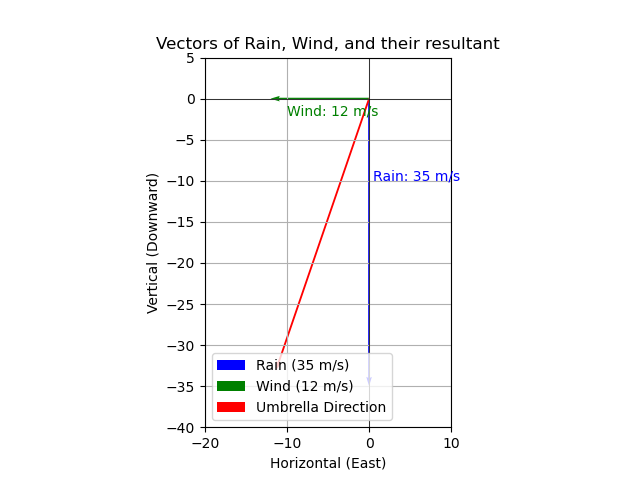
\includegraphics[width=0.7\linewidth]{figs/figure1.png}
   \caption{Plot showing the velocity vectors}
   \label{stemplot}
\end{figure}
\end{frame}
\subsection{Codes}
\begin{frame}
\frametitle{Codes}
The C code is:\\
 {\footnotesize
\begin{url}
https://github.com/Prahladha09/matgeo-1/blob/052f0e157e20ddbdbc2b9bb1bc67a4f8f578951b/assignment-1/codes/angle.c
\end{url}
}
The Python code is:\\
 {\footnotesize
\begin{url}
https://github.com/Prahladha09/matgeo-1/blob/052f0e157e20ddbdbc2b9bb1bc67a4f8f578951b/assignment-1/codes/plot.py
\end{url}
}
\end{frame}
\end{document}
